\Article{18}
\begin{center}\emph{Theorie des biquadratischen Restes $-1-2i$.}\end{center}
Der Modul $=m=a+bi$ sei so beschaffen, dass $a$ ungerade und $b$ gerade ist; außerdem setzen wir voraus, dass er eine Primzahl ist.

Die folgenden Schemata stellen den Dezidenten dar; von ihrer Identität überzeugt man sich leicht:
\begin{center}\resizebox{\textwidth}{!}{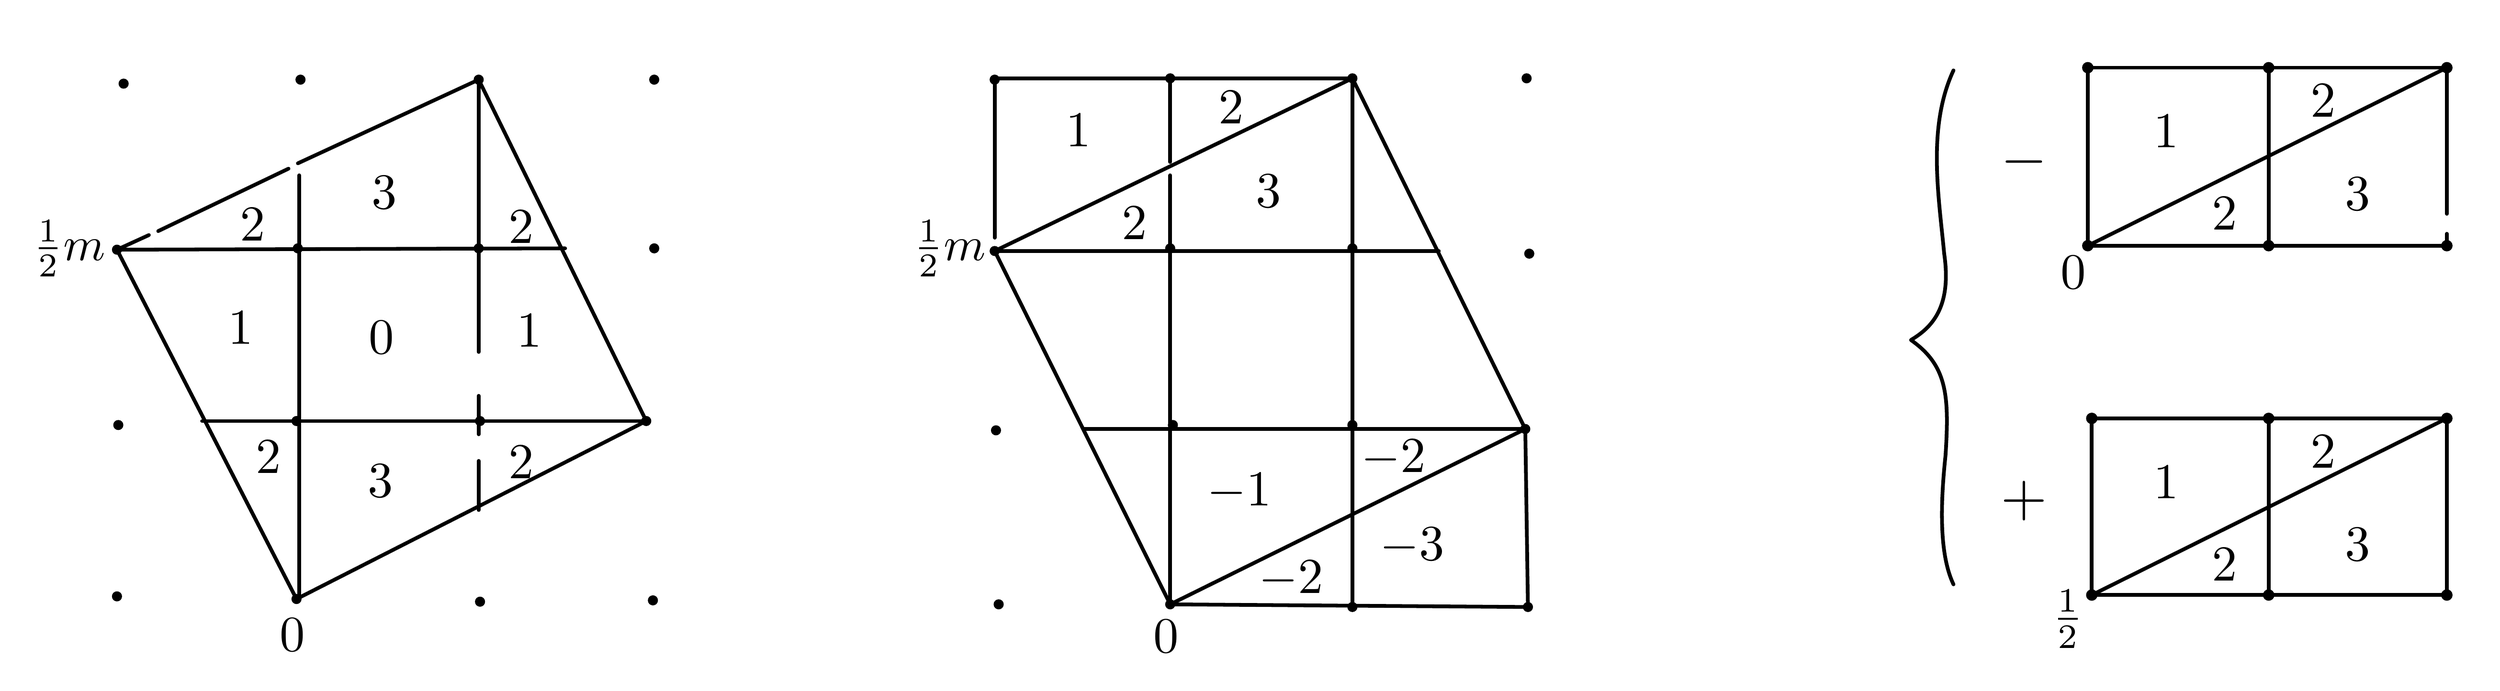
\begin{tikzpicture}[x=1bp,y=-1bp,line cap=round,line join=round]
\path[use as bounding box] (0,0) rectangle (1860,500);
\begin{pgfinterruptboundingbox}
\draw[line width=2.8bp] (78,178) -- (102,167);
\draw[line width=2.8bp] (109,164) -- (207,117);
\draw[line width=2.8bp] (214,113) -- (350,50) -- (476,307) -- (213,441) -- (78,178);
\draw[line width=2.8bp] (215,122) -- (215,441);
\draw[line width=2.8bp] (350,50) -- (350,255);
\draw[line width=2.8bp] (350,288) -- (350,317);
\draw[line width=2.8bp] (350,337) -- (350,374);
\draw[line width=2.8bp] (78,178) -- (415,177);
\draw[line width=2.8bp] (142,307) -- (476,307);
\fill (83,53) circle[radius=3.8bp];
\fill (216,50) circle[radius=3.8bp];
\fill (350,50) circle[radius=3.8bp];
\fill (482,50) circle[radius=3.8bp];
\fill (78,178) circle[radius=3.8bp];
\fill (214,177) circle[radius=3.8bp];
\fill (350,177) circle[radius=3.8bp];
\fill (482,177) circle[radius=3.8bp];
\fill (79,310) circle[radius=3.8bp];
\fill (213,307) circle[radius=3.8bp];
\fill (351,307) circle[radius=3.8bp];
\fill (476,307) circle[radius=3.8bp];
\fill (78,439) circle[radius=3.8bp];
\fill (213,441) circle[radius=3.8bp];
\fill (351,443) circle[radius=3.8bp];
\fill (481,442) circle[radius=3.8bp];
\node[inner sep=0pt,outer sep=0pt,anchor=center] at (180,159) {\scalebox{3.8}{\ensuremath{2}}};
\node[inner sep=0pt,outer sep=0pt,anchor=center] at (279,135) {\scalebox{3.8}{\ensuremath{3}}};
\node[inner sep=0pt,outer sep=0pt,anchor=center] at (382,161) {\scalebox{3.8}{\ensuremath{2}}};
\node[inner sep=0pt,outer sep=0pt,anchor=center] at (171,237) {\scalebox{3.8}{\ensuremath{1}}};
\node[inner sep=0pt,outer sep=0pt,anchor=center] at (277,244) {\scalebox{3.8}{\ensuremath{0}}};
\node[inner sep=0pt,outer sep=0pt,anchor=center] at (388,239) {\scalebox{3.8}{\ensuremath{1}}};
\node[inner sep=0pt,outer sep=0pt,anchor=center] at (192,334) {\scalebox{3.8}{\ensuremath{2}}};
\node[inner sep=0pt,outer sep=0pt,anchor=center] at (276,352) {\scalebox{3.8}{\ensuremath{3}}};
\node[inner sep=0pt,outer sep=0pt,anchor=center] at (382,338) {\scalebox{3.8}{\ensuremath{2}}};
\node[inner sep=0pt,outer sep=0pt,anchor=center] at (42,177) {\scalebox{3.6}{\ensuremath{\frac12 m}}};
\node[inner sep=0pt,outer sep=0pt,anchor=center] at (210,468) {\scalebox{3.8}{\ensuremath{0}}};
\draw[line width=2.8bp] (738,179) -- (1007,49) -- (1137,313) -- (870,445) -- cycle;
\draw[line width=2.8bp] (738,169) -- (738,49) -- (1007,49);
\draw[line width=2.8bp] (870,445) -- (1139,447) -- (1137,313);
\draw[line width=2.8bp] (870,49) -- (870,112);
\draw[line width=2.8bp] (870,122) -- (870,445);
\draw[line width=2.8bp] (1007,49) -- (1007,447);
\draw[line width=2.8bp] (738,179) -- (1072,179);
\draw[line width=2.8bp] (805,313) -- (1137,313);
\fill (738,50) circle[radius=3.8bp];
\fill (870,49) circle[radius=3.8bp];
\fill (1007,49) circle[radius=3.8bp];
\fill (1138,49) circle[radius=3.8bp];
\fill (738,179) circle[radius=3.8bp];
\fill (870,177) circle[radius=3.8bp];
\fill (1007,177) circle[radius=3.8bp];
\fill (1140,181) circle[radius=3.8bp];
\fill (739,314) circle[radius=3.8bp];
\fill (872,310) circle[radius=3.8bp];
\fill (1007,310) circle[radius=3.8bp];
\fill (1137,313) circle[radius=3.8bp];
\fill (741,445) circle[radius=3.8bp];
\fill (870,445) circle[radius=3.8bp];
\fill (1007,447) circle[radius=3.8bp];
\fill (1139,447) circle[radius=3.8bp];
\node[inner sep=0pt,outer sep=0pt,anchor=center] at (801,88) {\scalebox{3.8}{\ensuremath{1}}};
\node[inner sep=0pt,outer sep=0pt,anchor=center] at (843,158) {\scalebox{3.8}{\ensuremath{2}}};
\node[inner sep=0pt,outer sep=0pt,anchor=center] at (916,71) {\scalebox{3.8}{\ensuremath{2}}};
\node[inner sep=0pt,outer sep=0pt,anchor=center] at (944,134) {\scalebox{3.8}{\ensuremath{3}}};
\node[inner sep=0pt,outer sep=0pt,anchor=center] at (922,360) {\scalebox{3.8}{\ensuremath{-1}}};
\node[inner sep=0pt,outer sep=0pt,anchor=center] at (961,426) {\scalebox{3.8}{\ensuremath{-2}}};
\node[inner sep=0pt,outer sep=0pt,anchor=center] at (1038,335) {\scalebox{3.8}{\ensuremath{-2}}};
\node[inner sep=0pt,outer sep=0pt,anchor=center] at (1052,401) {\scalebox{3.8}{\ensuremath{-3}}};
\node[inner sep=0pt,outer sep=0pt,anchor=center] at (704,177) {\scalebox{3.6}{\ensuremath{\frac12 m}}};
\node[inner sep=0pt,outer sep=0pt,anchor=center] at (867,469) {\scalebox{3.8}{\ensuremath{0}}};
\draw[line width=2.8bp] (1459,43) .. controls (1439,86) and (1448,138) .. (1452,181) .. controls (1458,222) and (1442,237) .. (1427,246) .. controls (1454,265) and (1456,287) .. (1453,333) .. controls (1448,380) and (1450,411) .. (1459,430);
\draw[line width=2.8bp] (1830,151) -- (1830,41) -- (1560,41) -- (1560,175) -- (1830,175) -- (1830,166);
\draw[line width=2.8bp] (1696,41) -- (1696,175);
\draw[line width=2.8bp] (1560,175) -- (1830,41);
\fill (1560,41) circle[radius=4.3bp];
\fill (1696,41) circle[radius=4.3bp];
\fill (1830,41) circle[radius=4.3bp];
\fill (1560,175) circle[radius=4.3bp];
\fill (1696,175) circle[radius=4.3bp];
\fill (1830,175) circle[radius=4.3bp];
\node[inner sep=0pt,outer sep=0pt,anchor=center] at (1619,89) {\scalebox{3.8}{\ensuremath{1}}};
\node[inner sep=0pt,outer sep=0pt,anchor=center] at (1663,151) {\scalebox{3.8}{\ensuremath{2}}};
\node[inner sep=0pt,outer sep=0pt,anchor=center] at (1737,66) {\scalebox{3.8}{\ensuremath{2}}};
\node[inner sep=0pt,outer sep=0pt,anchor=center] at (1763,136) {\scalebox{3.8}{\ensuremath{3}}};
\draw[line width=2.8bp] (1563,305) -- (1830,305) -- (1830,438) -- (1563,438) -- cycle;
\draw[line width=2.8bp] (1696,305) -- (1696,438);
\draw[line width=2.8bp] (1563,438) -- (1830,305);
\fill (1563,305) circle[radius=4.3bp];
\fill (1696,305) circle[radius=4.3bp];
\fill (1830,305) circle[radius=4.3bp];
\fill (1563,438) circle[radius=4.3bp];
\fill (1696,438) circle[radius=4.3bp];
\fill (1830,438) circle[radius=4.3bp];
\node[inner sep=0pt,outer sep=0pt,anchor=center] at (1619,353) {\scalebox{3.8}{\ensuremath{1}}};
\node[inner sep=0pt,outer sep=0pt,anchor=center] at (1663,415) {\scalebox{3.8}{\ensuremath{2}}};
\node[inner sep=0pt,outer sep=0pt,anchor=center] at (1737,330) {\scalebox{3.8}{\ensuremath{2}}};
\node[inner sep=0pt,outer sep=0pt,anchor=center] at (1763,400) {\scalebox{3.8}{\ensuremath{3}}};
\node[inner sep=0pt,outer sep=0pt,anchor=center] at (1512,112) {\scalebox{4.5}{\ensuremath{-}}};
\node[inner sep=0pt,outer sep=0pt,anchor=center] at (1512,367) {\scalebox{4.5}{\ensuremath{+}}};
\node[inner sep=0pt,outer sep=0pt,anchor=center] at (1549,195) {\scalebox{3.8}{\ensuremath{0}}};
\node[inner sep=0pt,outer sep=0pt,anchor=center] at (1545,456) {\scalebox{3.7}{\ensuremath{\frac12}}};
\end{pgfinterruptboundingbox}
\end{tikzpicture}
}\end{center}

Der Kürze halber bezeichnen wir $S(x,x+\alpha,x+\alpha+\beta,x+\beta)$ mit $[x,\alpha,\beta]$, sodass
\[
\begin{aligned}
\relax
[x,\alpha,\beta]&=-[x,\beta,\alpha]=[x+\alpha,\beta,-\alpha]\\
&=-[x+\alpha,-\alpha,\beta]\\
&=[x+\alpha+\beta,-\alpha,-\beta]\\
&=-[x+\alpha+\beta,-\beta,-\alpha]
\end{aligned}
\]

\Needspace{16\baselineskip}
Setzt man ferner
\[
\frac{m}{-2-4i}=\frac{-a-2b}{10}+\frac{-b+2a}{10}i=Q
\]
\SourceLeaf{333}

so besteht der Dezident aus den folgenden acht Teilen:
\[
\begin{aligned}
\mathrm{I}&=[0,\tfrac12,-iQ]\\
-2\mathrm{II}&=-2[0,\tfrac12,Q]\\
\mathrm{III}&=+[Q,\tfrac12,-iQ]\\
\mathrm{IV}&=+[-iQ,\tfrac12,Q]\\
-3\mathrm{V}&=-3[Q,\tfrac12,Q]\\
-3\mathrm{VI}&=-3[2Q,\tfrac12,-iQ]\\
+2\mathrm{VII}&=+2[(1-i)Q,\tfrac12,Q]\\
+\mathrm{VIII}&=+[0,\tfrac12,\tfrac12im]
\end{aligned}
\]

Bezeichne $F$ einen beliebigen Elementarrest des Moduls $-1-2i$, so gilt
\[
\Sigma[2FQ,\tfrac12,iQ]=[0,-\tfrac12-i,\tfrac12im]
\]

Setzt man also für $F$ die Werte $0,1,i,-1,-i$ ein, so gilt
\[
\begin{array}{rll}
0={}&[0,\tfrac12,iQ]&=\mathrm{IX}\\
&+[2Q,\tfrac12,iQ]&=\mathrm{X}\pdot\\
&+[2iQ,\tfrac12,iQ]&=\mathrm{XI}\\
&+[-2Q,\tfrac12,iQ]&=\mathrm{XII}\\
&+[-2iQ,\tfrac12,iQ]&=\mathrm{XIII}\\
&-[0,-\tfrac12-i,\tfrac12im]&=-\mathrm{XIV}
\end{array}
\]

Man addiere dies zum vorigen Wert des Dezidenten. Aus dieser Verbindung ergeben sich die folgenden Resultate:

(1) Da $(1+2i)Q+\frac12$ eine ganze Zahl ist, gilt
\[
\begin{aligned}
\mathrm{XI}&=[-Q-\tfrac12,\tfrac12,iQ]= -[-Q,-\tfrac12,iQ]\\
&=-[Q,\tfrac12,-iQ]
\end{aligned}
\]
also
\[
\mathrm{III}+\mathrm{XI}=0
\]

(2) Wir fassen $\mathrm{IV},-3\mathrm{V},\mathrm{X},\mathrm{XIII}$ auf folgende Weise zusammen:
\[
\begin{aligned}
\mathrm{IV}&=+[-2Q+\tfrac12i,\tfrac12,Q]=[-2iQ-\tfrac12,\tfrac12i,iQ]\\
\mathrm{V}'&=-[2Q,+\tfrac12,-Q]=-[-2iQ,-\tfrac12i,iQ]\\
\mathrm{X}&=[+iQ-\tfrac12i,\tfrac12,iQ]\\
&=[-iQ+\tfrac12i,-\tfrac12,-iQ]=[-2iQ-\tfrac12+\tfrac12i,\tfrac12,iQ]\\
\mathrm{XIII}&=[-2iQ,\tfrac12,iQ]
\end{aligned}
\]

\SourceLeaf{334}

Das gesamte Ergebnis aus diesen Teilen ist also
\[
\begin{aligned}
&-4\mathrm{V}\\
&+R(-2iQ)-R(-iQ)-I(-2iQ)+I(-iQ)\\
&-\text{Quadr. }[-2iQ-\tfrac14+\tfrac14i]\\
&+\text{Quadr. }[-2iQ+\tfrac14-\tfrac14i]
\end{aligned}
\]

(3) Fasst man $\mathrm{I},-2\mathrm{II},-3\mathrm{VI},+2\mathrm{VII},+\mathrm{IX},+\mathrm{XII}$ zusammen, so ergibt sich
\[
\begin{aligned}
\mathrm{I}&=[0,\tfrac12,-iQ]\\
\mathrm{II}&=[0,-\tfrac12i,-iQ]\\
\mathrm{VI}&=[iQ-\tfrac12i,\tfrac12,-iQ]=[\tfrac12-\tfrac12i,-\tfrac12,iQ]\\
&=[-\tfrac12+\tfrac12i,\tfrac12,-iQ]\\
\mathrm{VII}&=[-Q-\tfrac12i,\tfrac12,Q]=[-\tfrac12+\tfrac12i,-\tfrac12,-Q]\\
&=[+\tfrac12+\tfrac12i,-\tfrac12i,-iQ]\\
\mathrm{IX}&=[0,-\tfrac12,-iQ]\\
\mathrm{XII}&=[-iQ+\tfrac12i,\tfrac12,iQ]=[\tfrac12+\tfrac12i,-\tfrac12,-iQ]
\end{aligned}
\]
\[
\begin{aligned}
={}&+4\mathrm{I}-4\mathrm{II}-4\mathrm{VI}+4\mathrm{XII}\\
&-I(\tfrac12i)+I(-iQ+\tfrac12i)+I0-I(-iQ)-2R0+2R(-iQ)\\
&+2\text{Quadr. }(-iQ+\tfrac14+\tfrac14i)\\
={}&4\mathrm{I}-4\mathrm{II}-4\mathrm{VI}+4\mathrm{XII}\\
&+R(-1-2i)Q-R(-2iQ)-I(-iQ)+2R(-iQ)\\
&+2\text{Quadr. }(-2iQ+\tfrac14+\tfrac14i)
\end{aligned}
\]

Dies alles zusammen ergibt folglich
\[
\begin{aligned}
&+4\mathrm{I}-4\mathrm{II}-4\mathrm{V}-4\mathrm{VI}+4\mathrm{XII}+\tfrac12(a-1)-\tfrac12b\\
&+\text{Quadr. }(-2iQ+\tfrac14-\tfrac14i)\\
&+2\text{Quadr. }(-2iQ+\tfrac14+\tfrac14i)\\
&-\text{Quadr. }(-2iQ-\tfrac14+\tfrac14i)
\end{aligned}
\]

Schließlich ergibt sich $\mathrm{VIII}-\mathrm{XIV}=\frac12(a-1)+\frac12b$.
Da die drei Quadratteile dem Dezidenten von $\frac{m}{-1-2i}$ gleich sind, gilt also
\[
\text{Dez. }\frac{-1-2i}{m}\equiv a-1+\text{Dez. }\frac{m}{-1-2i}\quad\text{Was zu beweisen war.}
\]

Wahrscheinlich lässt sich der Beweis noch erheblich dadurch vereinfachen, dass
\[
\text{Dez. }\frac{1+2i}{m}=\vcenter{\hbox{\resizebox{.35\textwidth}{!}{\begin{tikzpicture}[x=1bp,y=-1bp,line cap=round,line join=round]
\path[use as bounding box] (0,0) rectangle (620,220);
\begin{pgfinterruptboundingbox}
\draw[line width=2.1bp] (147,35) -- (485,32) -- (213,173) -- cycle;
\node[inner sep=0pt,outer sep=0pt,anchor=east] at (138,34) {\scalebox{2.6}{\ensuremath{\frac12(1+i)m}}};
\node[inner sep=0pt,outer sep=0pt,anchor=west] at (494,32) {\scalebox{2.6}{\ensuremath{(-1+i)m}}};
\node[inner sep=0pt,outer sep=0pt,anchor=center] at (205,194) {\scalebox{3.6}{\ensuremath{0}}};
\end{pgfinterruptboundingbox}
\end{tikzpicture}
}}}
\]

\SourceLeaf{335}

\Article{19}
Durch Induktion wurde Folgendes gefunden:
\[
\begin{aligned}
\text{Dez. }\frac{a-bi}{a+bi}&\equiv\frac{aa+2ab-1}{4},& a&\equiv1\ (\mathrm{mod.}\ 4)\\
&\equiv\frac{aa+2ab+2bb-1}{4},&a+bi&\equiv1\ (\mathrm{mod.}\ 2+2i)
\end{aligned}
\]

Damit hängt Folgendes zusammen:
Es sei $aa+bb=p$ (Primzahl), $a\equiv1\ (\mathrm{mod.}\ 4)$
\[
\begin{aligned}
1\pdot2\pdot3\mathinner{.\,.\,.\,.\,.\,.\,.\,.\,.\,.\,.}\tfrac14(p-1)&\equiv\alpha\ \mathrm{mod.}p\\
\tfrac14(p+3)\pdot\tfrac14(p+7)\ldots\tfrac12(p-1)&\equiv\beta\\
\tfrac12(p+1)\pdot\tfrac12(p+3)\ldots\tfrac34(p-1)&\equiv\gamma\\
\tfrac14(3p+1)\mathinner{.\,.\,.\,.\,.\,.\,.\,.\,.}\ p-1&\equiv\delta
\end{aligned}
\]
so gilt
\[
\begin{aligned}
\alpha&\equiv\delta,&\beta&\equiv\gamma&\text{wenn }\tfrac12b\text{ gerade}\\
\alpha&\equiv-\delta,&\beta&\equiv-\gamma&\text{wenn }\tfrac12b\text{ ungerade}
\end{aligned}
\]
\[
\begin{gathered}
\pm\alpha\beta\equiv i,\quad\pm\beta\beta\equiv2b,\quad\frac\beta\alpha\equiv2a,\\
\frac\beta{1+\alpha\beta}\equiv\surd a,\quad\tfrac12\beta(1-\alpha\beta)\equiv\surd a
\end{gathered}
\]

Es kommt demnach nur noch darauf an, die Dezidenten bei reellen Resten zu bestimmen.
\[
\begin{gathered}
a^{\frac14bb}\pdot b^{\frac14(aa-1)}\equiv1\ (\mathrm{mod.}\ (aa+bb))\\
\text{wenn }a\equiv1)(\mathrm{mod.}\ 4)\quad b\text{ gerade}\quad aa+bb\text{ Primzahl}
\end{gathered}
\]

Will man nur mit reellen Zahlen arbeiten, so kommt es auf den folgenden Hauptsatz an. Es sei $a-1$ durch $4$ und $b$ durch $2$ teilbar; $a$ und $b$ seien ohne gemeinsamen Teiler, und $k$ bezeichne die Zahlen $1,2,3\ldots aa+bb-1$.
Es sei
\begin{list}{}{\setlength{\labelwidth}{1.5em}\setlength{\leftmargin}{2em}}
\item[$\alpha$] die Anzahl aller Werte von $k$, für die die kleinsten Reste von $ak,\allowbreak bk,\quad\allowbreak aak,\quad\allowbreak abk$ alle zwischen $0$ und $\frac12(aa+bb)$ liegen
\item[$\beta$] $ak,bk,\quad aak,-abk$
\item[$\gamma$] $ak,bk,-aak,-abk$
\item[$\delta$] $ak,bk,-aak,\quad abk$
\end{list}
Dann ist $\beta+2\gamma+3\delta-\frac14(aa-1)$ durch $4$ teilbar.
\BookRule{.35\textwidth}
